\ifx\allfiles\undefined
\documentlecture[12pt, a4paper, oneside, UTF8]{ctexbook}  %  这一句是新增加的
\usepackage[dvipsnames]{xcolor}
\usepackage{amsmath}   % 数学公式
\usepackage{graphicx}
\usetikzlibrary{arrows, calc, decorations.pathmorphing}
\allowdisplaybreaks % 允许公式跨页换行
\newcommand{\pa}{\partial}
\newcommand{\mathminus}{\!\!-\!\!} % 数学环境连字符
\newcommand{\vsup}[1]{\raisebox{-0.1ex}{$\scriptstyle #1$}}
\newcommand{\lsup}[1]{\raisebox{-0.85ex}{$\scriptstyle #1$}}
\definecolor{b1}{RGB}{0,191,255}



\begin{document}
%
 % 单独编译时,其实不用编译封面目录之类的,如需要不注释这句即可
\else
\fi
%  ↓↓↓↓↓↓↓↓↓↓↓↓↓↓↓↓↓↓↓↓↓↓↓↓↓↓↓↓ 正文部分
\chapter{concise review of basic concepts and definitions}
\section{lecture 1}
\begin{defn}
\par\indent
\begin{enumerate}
    \item \textcolor{b1}{system}:\;
    set of constituents\;(\textbf{not subjected to forces that depend on coordinates of other external constituents})
    \item \textcolor{b1}{property}:\; 
    the system at time \( t \), yields a numerical result \( P(t) \)\;(\textbf{not depend on other instants of time})
    \item \textcolor{b1}{state}:\; 
    the state of the system at time \( t \) is the set of
     (a) the values of the amounts of all constituents,
     (b) the values of the external and internal, and
     (c) the values of all the conceivable properties
\[ A(t) = \{ n_1(t), \cdots, n_r(t), \beta_1(t), \cdots, \beta_s(t), P_1(t), P_2(t), \cdots \} 
\qquad A_1:=A(t_1)\]
\begin{itemize}
    \item \( r\) number of different constituents
    \item \( s\) number of parameters
\end{itemize}
\begin{add}
    Time evolution of the state of the system
    General equation of motion:
\[ \frac{dA(t)}{dt} = f[A(t), \text{forces}(t)] \rightarrow A(t_1)\]

Two theorems of the equation of motion hold for all (well-defined) systems:
\begin{enumerate}
\item First Theorem (Conservation of Linear Momentum)
\item Second Theorem (Conservation of Angular Momentum)
\end{enumerate}
\begin{zhu}
    "well-defined systems"(良好定义的系统)指的是那些能够用明确的数学框架(如拉格朗日力学或哈密顿力学)来描述的系统。
\end{zhu}
\end{add}
    \item \textcolor{b1}{process}:\; 
    specified by
    \begin{itemize}
    \item The initial state of the system
    \item The final state of the system
    \item The effects produced by the interactions with other systems
    \end{itemize}
    \[ A_1 \rightarrow A_2 \]
    \begin{zhu}
        A process simplifies the description of time evolution by abstracting the behavior of a system 
        into a series of state changes over time. 
        
        Instead of detailing \textbf{every instantaneous configuration 
        or interaction}, a process focuses on the overall transformation \textbf{from an initial state to a final state}.
    \end{zhu}
\end{enumerate}
\end{defn}
\begin{defn}
    \par\indent
    \begin{itemize}
        \item Spontaneous Process (no effects on the environment)
        \item Weight Process (external effects are only ``mechanical''(mechanical work))
    \end{itemize}
    \begin{zhu}
    \par\indent
\begin{itemize}
    \item Spontaneous Process 强调了热力学中的不可逆性和能量转换的方向性,将力学中的能量概念与热力学中的熵增联系起来。
    \item Weight Process 将力学中的功与热力学中的能量守恒联系起来。
\end{itemize}
    \end{zhu}
\end{defn}
\begin{law}
    First Law (a unique form):
    \begin{itemize}
    \item \textbf{Assertion 1:} any pair of states \( A_1 \) and \( A_2 \) with 
    compatible values of the amounts of constituents and the parameters of 
    a (well-defined) system \( A \) \textbf{can always be interconnected by} means of a weight process.
    \item \textbf{Assertion 2:} the product \( mg(z_2 - z_1) \) assumes \textbf{the same value for all weight processes} that connect the two given states \( A_1 \) and \( A_2 \).
    \end{itemize}
\end{law}
\begin{corollary}
    Consequences of the First Law:
    \begin{enumerate}
        \item Additivity of energy
        \item Conservation of energy
        \item Exchangeability of energy via interactions
        \item Energy balance equation for a process for system \( A \) (the usual form of the First Law)
    \end{enumerate}
\end{corollary}
\begin{minipage}{0.85\textwidth}
    \centering
    \captionof{table}{Comparison of Steady, Unsteady, Equilibrium, and Nonequilibrium States}
    \begin{tabular}{|p{4cm}<{\centering}|p{4cm}<{\centering}|p{5cm}<{\centering}|}
        \hline
            ~ & ...because of external interactions & ...even if external interactions are turned off \\ 
        \hline
            The state changes with time... & Unsteady state  & Nonequilibrium state \\
        \hline
            The state does not change with time... & Steady state  & Equilibrium state \\ 
        \hline
    \end{tabular}
\end{minipage}
\begin{defn}
    Unstable equilibrium,
    Metastable equilibrium,
Stable equilibrium and

Nonequilibrium
    \par\indent
\begin{minipage}{0.8\textwidth}
    \centering
    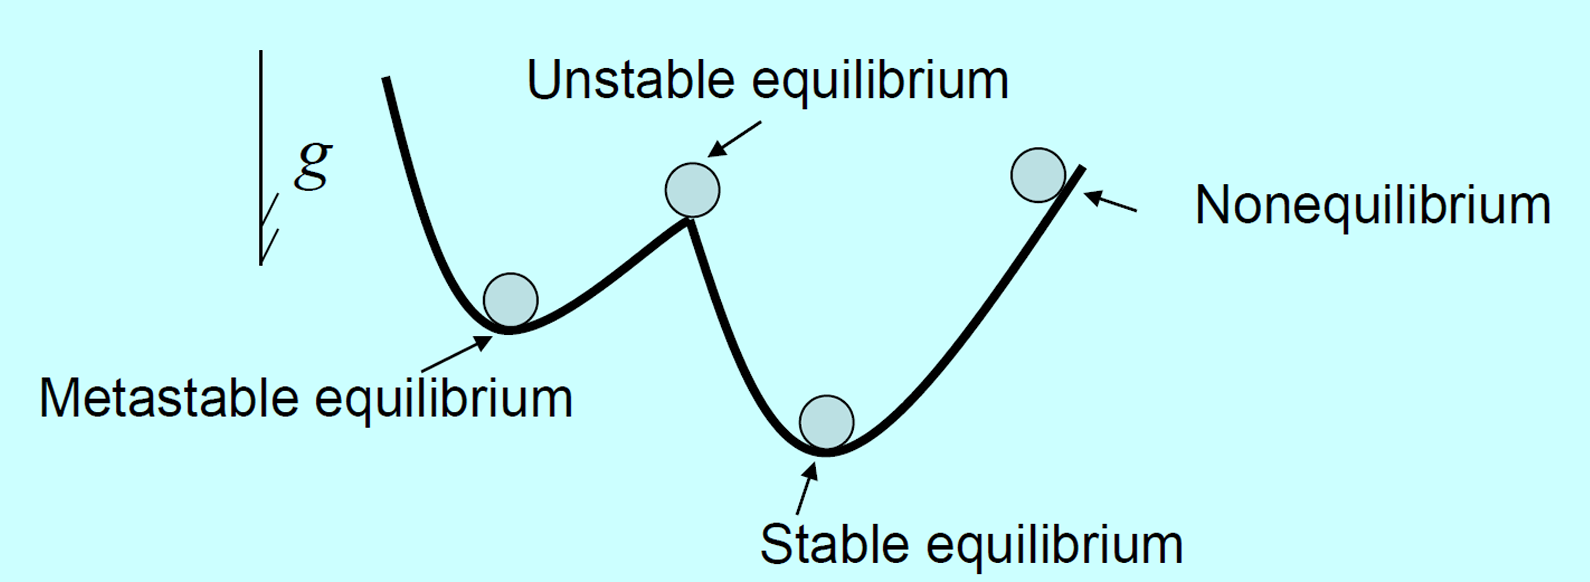
\includegraphics[width=0.75\textwidth]{chap1/1.1.png}
\end{minipage}
\end{defn}
\begin{law}
    Second Law:

\begin{itemize}
\item \textbf{Assertion 1:} in the subset of states of a system compatible with 
given values of the amounts of constituents \( n \) and of the parameters \( \beta \), 
there is always \textbf{one and only one SES} for each value of the energy \( E \).  
\item \textbf{Assertion 2:} Starting from any state of the system, it is always possible, 
\textbf{through a reversible weight process}, to reach a SES with arbitrarily fixed, 
\textbf{compatible values of the amounts} of constituents and the parameters.
\end{itemize}
\begin{zhu}
    \par\indent
    \begin{itemize}
    \item \textbf{Mechanics:} One and only one: the stable equilibrium state with minimum energy, \( E_g (n, \beta) \). 
    \item \textbf{Thermodynamics:} One for every value of the energy \( E \)
\end{itemize}
\end{zhu}
\end{law}
\section{lecture 2}
\begin{thm}\label{cfsl1}
    Consequences of First \& Second Law (p\pageref{cfsl2}\;,\; p\pageref{cfsl3})
    \begin{itemize}
        \item Kelvin-Planck statement: impossibility of perpetual motion of the second kind
        
        (It is impossible to extract mechanical energy without other effects from a system initially in a stable equilibrium state)
        \item Clausius statement: Conditions for the spontaneous exchange of energy between systems initially in stable equilibrium states but not in mutual equilibrium
    \end{itemize}
\begin{proof}
    the Kelvin-Planck Statement of the Second Law

\textbf{Ab absurdo:} assume that a PMM2 be possible (further assume, for simplicity of proof here, 
that system \( A \) is composed of two separate parts).

The final states is different from the initial one, and the initial
one was a Steady Equilibrium State.
\end{proof}
\begin{zhu}
    Synonyms of ab absurdo include “reductio ad absurdum,” “proof by contradiction,” and “proof by absurdity.”
\end{zhu}
\end{thm}
\begin{defn}
    The \textbf{adiabatic availability} \( \Psi_1 \) of system \( A \) in state \( A_1 \) 
    measures \textbf{the maximum amount of energy} that \textbf{can be transferred} from the system 
    to a weight in a weight process for \( A \) starting from state \( A_1 \).
    \(\Psi_1=E_1-E_{s1}\)
\end{defn}
\begin{thm}
    Adiabatic availability is a property, but it is \(\underset{\text{lack of utility}}{\text{not additive}}\).
\end{thm}
\begin{defn}
    Mutual stable equilibrium
      
    Two systems \( A \) and \( B \) are in mutual stable equilibrium if their respective states are such that the composite system \( AB \) is in a stable equilibrium state.
\end{defn}
\begin{defn}
    A system \( R \) that in any of its stable equilibrium states is 
    in mutual equilibrium with a given system \( C \) in a given state \( CR \).
    \begin{explain}
        A thermal reservoir, denoted as \(R\), 
        is a system that can exchange energy (typically heat) with another system 
    \(C\) without undergoing any significant change in its own properties.     
    \end{explain}
    \begin{zhu}
        Thermal reservoirs are often used as heat sources or sinks in thermodynamic processes. 
    \end{zhu}
\end{defn}
\begin{proposition}
    It can be proved that the ratio:
\[ \frac{(E_{s2rev}^R - E_{s1}^R)_{A_1 R_{s1} \underset{w,rev}{\rightarrow} A_2 R_{s2rev}}}
{(E_{s2rev}^{R^\circ } - E_{s1}^{R^\circ })_{A_1 R_{s1}^\circ \underset{w,rev}{\rightarrow} A_2 R^\circ _{s2rev} }} 
\]
\begin{itemize}
    \item is positive, 
    \item is independent of \(\begin{cases}
    \text{the initial states}\; R_{s1}, \;R^\circ_{s1}\; \text{of the reservoirs,}\\
    \text{the choice of the auxiliary system} \;A\; \text{and of its states} \; A_1 \;\text{and}\; A_2 , 
    \end{cases}\)
    \item depends solely on the pair of reservoirs \( R \) and \( R^\circ \),
    \item is a dimensionless number.
\end{itemize}
\end{proposition}
\begin{defn}
    property temperature of reservoir \(R\)
\begin{gather*}
T_R=T_{R^\circ}\frac{(E_{s2rev}^R - E_{s1}^R)_{A_1 R_{s1} \underset{w,rev}{\rightarrow} A_2 R_{s2rev}}}
{(E_{s2rev}^{R^\circ } - E_{s1}^{R^\circ })_{A_1 R_{s1}^\circ \underset{w,rev}{\rightarrow} A_2 R^\circ _{s2rev} }} 
\\
\frac{(E_{s2rev}^R - E_{s1}^R)_{A_1 R_{s1} \underset{w,rev}{\rightarrow} A_2 R_{s2rev}}}{T_R}
=\frac{(E_{s2rev}^{R^\circ } - E_{s1}^{R^\circ })_{A_1 R_{s1}^\circ \underset{w,rev}{\rightarrow} A_2 R^\circ _{s2rev}}}{T_{R^\circ}}
\end{gather*}

The ratio 
\begin{itemize}
    \item is independent of reservoir \( R \) and of its initial state \( R_{s1} \)
    \item It depends therefore only on system \( A \) and the pair of states \( A_1 \) and \( A_2 \)
\end{itemize}
\end{defn}
\begin{defn}
    property entropy
    
    The ratio:
\[
\frac{\left(E_{s0\text{rev}}^R - E_{s1}^R\right)_{A_1 R_{s1} \underset{w,rev}{\rightarrow} A_0 R_{s0\text{rev}}}}{T_R}
\]
\begin{itemize}
    \item is independent of reservoir \( R \) and of its initial state \( R_{s1} \)
    \item It depends therefore only on system \( A \) and the pair of states \( A_1 \) and \( A_0 \)
\end{itemize}
\[
S_1 = S_0 + \frac{\left(E_{s0\text{rev}}^R - E_{s1}^R\right)_{A_1 R_{s1} \underset{w,rev}{\rightarrow} A_0 R_{s0\text{rev}}}}{T_R}
\]
\end{defn}
\begin{defn}
    Available Energy w.r.t. a thermal reservoir

    Given state \( A_1 \) and the reservoir \( R \), 
    the maximum weight lift obtains when \( A \) ends 
    in state \( A_R \) and the standard weight process for \( AR \) is reversible.
    \[\Omega_1^R=(E_1-E_R)+(E^R_{s1}-E^R_{sRrev})
    =(E_1-E_R)-(E^R_{sRrev}-E^R_{s1})=(E_1-E_R)-T_R(S_1-S_R)\]
    We call it \textbf{available energy of \(A\) in state \(A_1\) w.r.t. a thermal reservoir \(R\)}.
\end{defn}
\begin{thm}\label{cfsl2}
    Consequences of the (First\&) Second Law (p\pageref{cfsl1}\;,\; p\pageref{cfsl3})
    \begin{itemize}
        \item supports the definition of property adiabatic availability
        \item supports the definition of property temperature of a thermal reservoir
        \item supports the definition of property entropy
        \item The entropy is \textbf{a linear function} of that part of the energy of the system which  
        is unavailable with respect to the reservoir, \textbf{the constant of proportionality} being \textbf{the  
        inverse of the temperature} of the reservoir.
        \begin{center}
            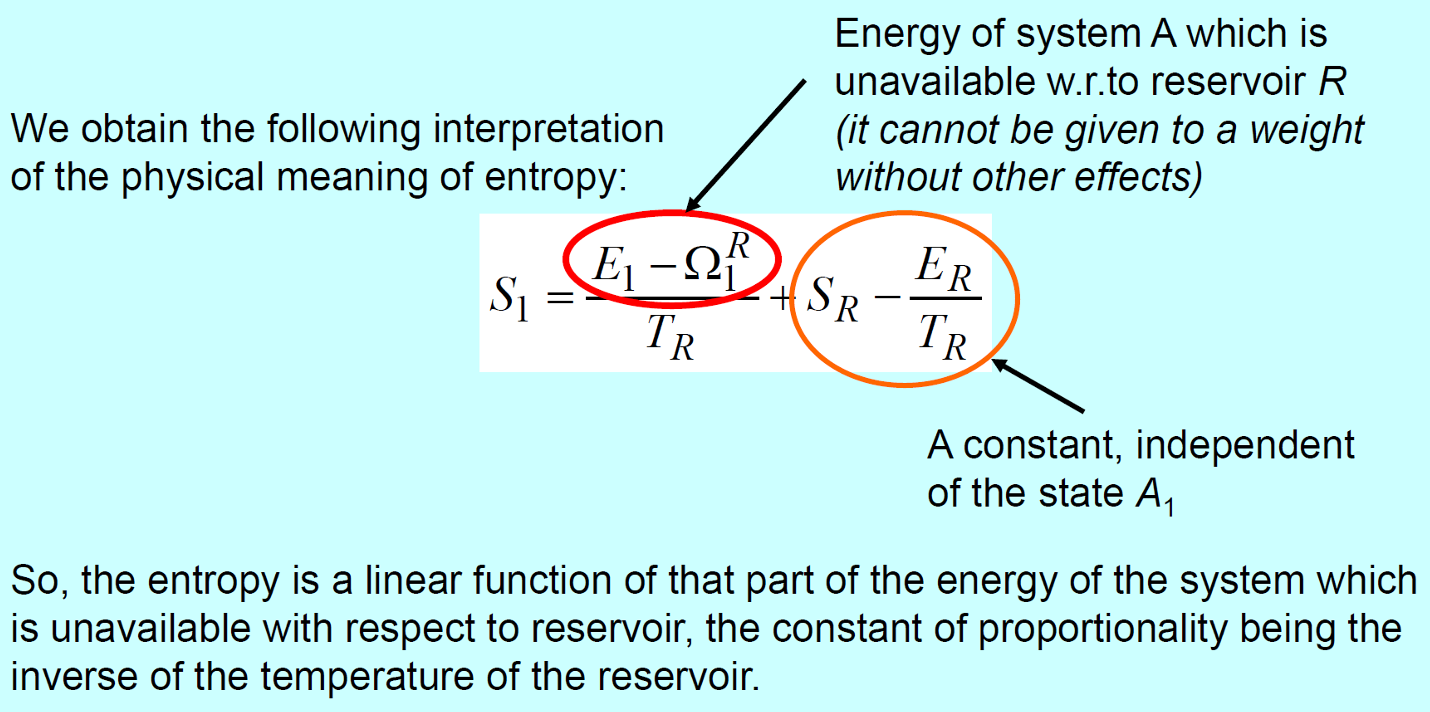
\includegraphics[width=0.7\textwidth]{chap1/2.1.png}
        \end{center}
        \item additivity of entropy 
        \item exchangeability of entropy via interactions
        \item principle of entropy non\textminus decrease in a weight process
    \end{itemize}
\end{thm}
\begin{corollary}
    Criteria for the reversibility of a weight process
    \begin{itemize}
        \item \textbf{Reversible iff:} \( E_2 - \Psi_2 = E_1 - \Psi_1 \qquad
        E_2 - \Omega^R_2 = E_1 - \Omega^R_1 \qquad S_2=S_1\)
        \item \textbf{Irreversible iff:} \( E_2 - \Psi_2 \geq E_1 - \Psi_1 \qquad
        E_2 - \Omega^R_2 \geq E_1 - \Omega^R_1 \qquad S_2\geq S_1 \)
        \item \textbf{Impossible iff:} \( E_2 - \Psi_2 \leq E_1 - \Psi_1 \qquad
        E_2 - \Omega^R_2 \leq E_1 - \Omega^R_1 \qquad S_2\leq S_1 \)
    \end{itemize}
\end{corollary}
\begin{thm}
    
\end{thm}

\textbf{Maximum entropy principle:} Among all the states with the same given values of the amounts of constituents, the parameters, and \textbf{the energy}, only the stable equilibrium state has the maximum value of the entropy.

\textbf{Minimum energy principle:} Among all the states with the same given values of the amounts of constituents, the parameters, and \textbf{the entropy}, only the stable equilibrium state has the minimum value of the energy.
\begin{add}
    \textbf{非平衡态系统中最小能量原理失效}:
        \begin{itemize}
            \item 传统热力学中,系统趋向能量最低态的前提是孤立或平衡条件。
            \item 非平衡态系统的能量可能被外部驱动力“泵入”,导致能量高于平衡态(如生物细胞的主动运输)。
        \end{itemize}
\end{add}
\begin{thm}\label{cfsl3}
    Consequences of the (First\&) Second Law (p\pageref{cfsl1}\;,\; p\pageref{cfsl2})
\begin{itemize}
    \item State Principle
    
    Among all the states with the same given values of the amounts of constituents, the parameters, 
    and the energy, one and only one is a stable equilibrium state (Second Law) and 
    therefore the value of any property is uniquely determined by the values of 
    the amounts of constituents, the parameters, and the energy.
    \[
    P = P(E, n_1, \ldots, n_r, \beta_1, \ldots, \beta_s)
    \] 
    \item Gibbs relation
    \begin{itemize}
        \item 
        \(
        S = S(E, V, n_1, \dots, n_r)
        \),        
        Gibbs relation (entropy form):
\[
dS = \frac{1}{T} dU + \frac{P}{T} dV - \sum_i \frac{\mu_i}{T} dn_i
\]
        \item 
        \(
        E = E(S, V, n_1, \dots, n_r)
        \),        
        Gibbs relation (energy form):
        \[
        dE = T dS - P dV + \sum_i \mu_i dn_i
        \]
    \end{itemize}
    \begin{add}
        通过诺特定律,Gibbs 关系的能量形式和熵形式可以统一解释为:
\begin{itemize}
    \item 能量形式:时间平移对称性生成的守恒内能 \(E\),描述了系统的守恒性质。
    \item 熵形式:熵最大化原理,描述了系统在自发过程中熵的变化方向。
\end{itemize}
        两种形式通过 Legendre 变换和对偶对称性紧密关联。
    \begin{zhu}
        热力学中常见的对称性:

    时间平移对称性 $\Rightarrow$ 能量守恒,
    空间均匀性 $\Rightarrow$ 压强平衡,
    粒子数守恒 $\Rightarrow$ 化学势平衡。
    \end{zhu}
    \end{add}
\end{itemize}
\end{thm}
\begin{defn}
    \par\indent
    \begin{itemize}
        \item The (absolute) temperature is defined by  
        \[
        T = \left( \frac{\partial E}{\partial S} \right)_{\vec{n}, V} \quad \text{or} \quad \left( \frac{\partial S}{\partial E} \right)_{\vec{n}, V} = \frac{1}{T}
        \]          
        \item The chemical potential of the \(i\)-th constituent is defined by  
        \[
        \mu_i = \left( \frac{\partial E}{\partial n_i} \right)_{S, V} \quad \text{or} \quad \left( \frac{\partial S}{\partial n_i} \right)_{E, V} = -\frac{\mu_i}{T}
        \]          
        \item The pressure is defined by  
        \[
        p = - \left( \frac{\partial E}{\partial V} \right)_{S, \vec{n}} \quad \text{or} \quad \left( \frac{\partial S}{\partial V} \right)_{E, \vec{n}} = \frac{p}{T}
        \]
    \end{itemize}
\end{defn}
\section{lecture 3}
\begin{proposition}
    Necessary Conditions for Mutual Equilibrium
    \begin{itemize}
        \item \((T_1=T_2)\)
        \textbf{Equality of the temperatures} of the two systems is a necessary condition for mutual equilibrium if the two systems can exchange \textbf{energy}.
        \item \((p_1=p_2)\)
        \textbf{Equality of the pressures} of the two systems is a necessary condition for mutual equilibrium if the two systems can exchange \textbf{volume}.
        \item \((\mu_{i,1} = \mu_{i,2})\)
        \textbf{Equality of the chemical potentials of the \(i\)-th constituent} in the two systems is a necessary condition for mutual equilibrium if the two systems can exchange \textbf{the \(i\)-th constituent}.
    \end{itemize}
\end{proposition}
\begin{minipage}{0.8\textwidth}
    \centering
    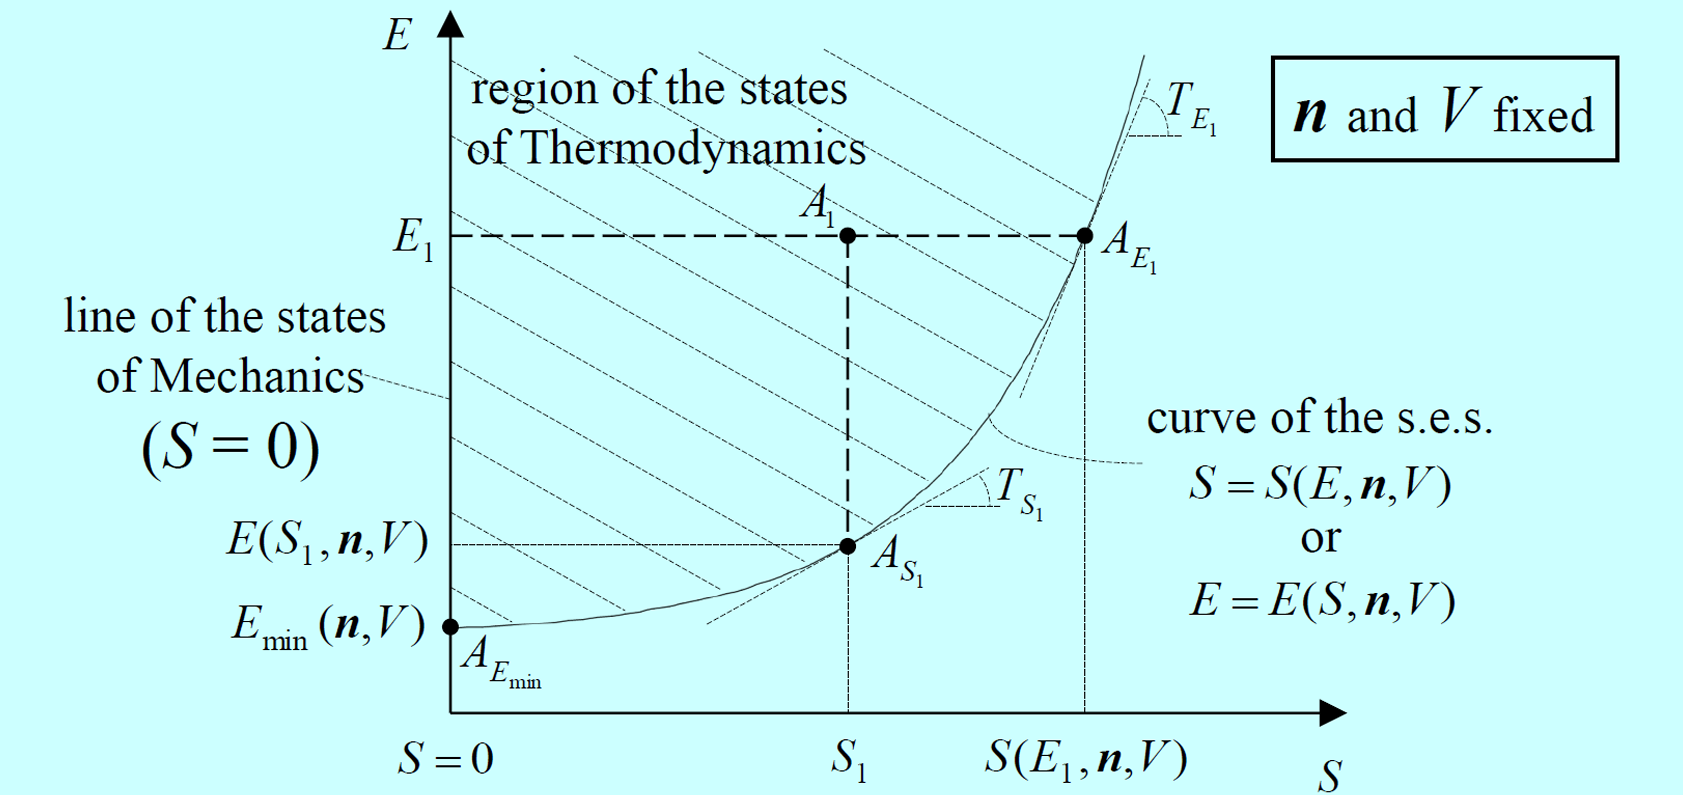
\includegraphics[width=0.75\textwidth]{chap1/3.1.png}
    \captionof{figure}{Representation of notSES and SES}
\end{minipage}
\begin{defn}
    negative temperatures \(T_{N1}\)

\begin{minipage}{0.8\textwidth}
    \centering
    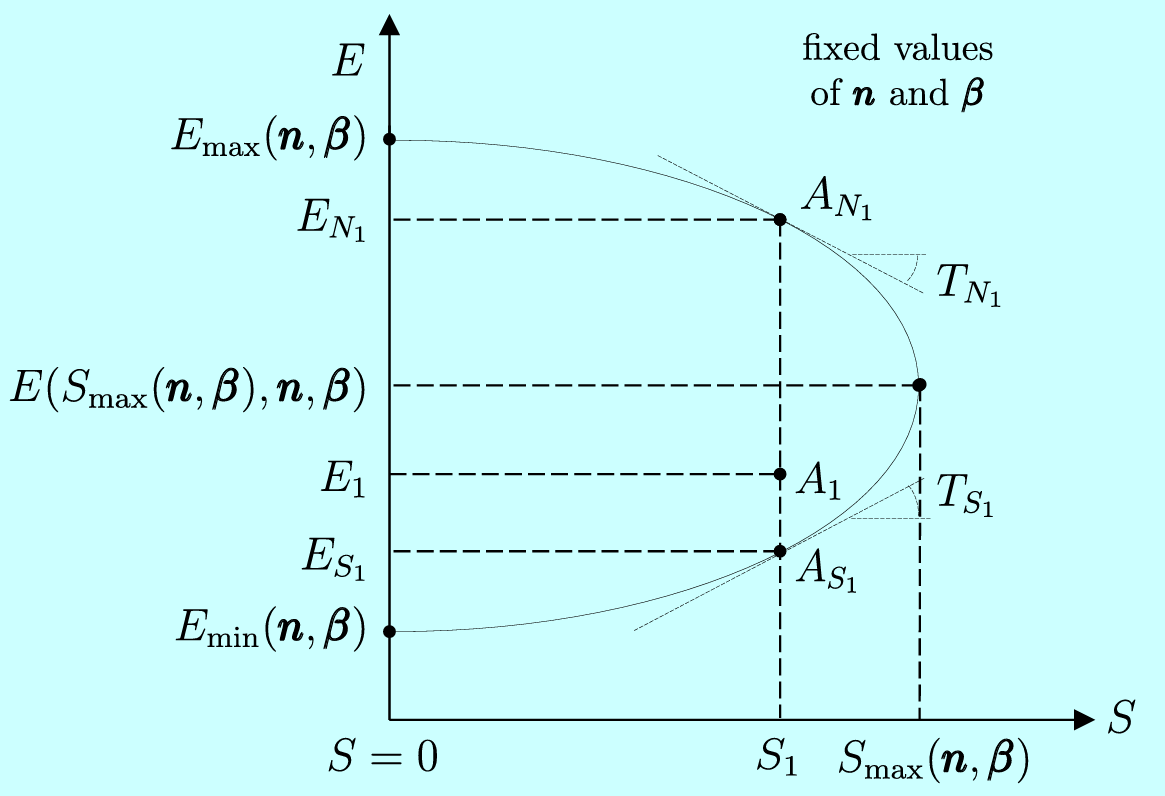
\includegraphics[width=0.5\textwidth]{chap1/3.2.png}
    \captionof{figure}{Special systems with upper bounded energy}
\end{minipage}
\end{defn}
\section{lecture 4}
\begin{thm}
    \indent
    \begin{itemize}
        \item To extract energy from a system in a s.e.s., we must also extract entropy:
        \[
        S_{s1} - S_{s2} > (E_{s1} - E_{s2}) / T_{s1}
        \]
        \item To give entropy to a system in a s.e.s., we must also give energy:
        \[
        E_{s2} - E_{s1} > T_{s1}(S_{s2} - S_{s1})
        \]
    \end{itemize}
    \begin{add}
阴阳动态平衡与热力学公式的哲学对应

\begin{itemize}
    \item \textbf{能量与熵的不可分割性 (万物负阴而抱阳) }  
    \[
    S_{s1} - S_{s2} > \frac{E_{s1} - E_{s2}}{T_{s1}}
    \]
    \textit{哲学内涵}:能量(阳)显化为外在功用时,系统内禀的微观状态自由度(阴)必须同步减少,以熵的隐性耗散为代价。
    \[
    E_{s2} - E_{s1} > T_{s1}(S_{s2} - S_{s1})
    \]
    \textit{哲学内涵}:熵增(阴)代表系统微观状态自由度的扩展,而能量输入(阳)则是维持这种扩展的必要动力。
    \item \textbf{动态平衡 (冲气为和) }  
    
    系统稳态(s.e.s.)下的状态迁移需满足:
    \[
    \Delta E > T\Delta S \quad \text{或} \quad \Delta S > \frac{\Delta E}{T}
    \]
    \textit{哲学内涵}:阴阳消长需通过能量\textminus 熵交换(冲气)达成新平衡。不等式方向表明:
    \begin{itemize}
        \item 当系统释放能量(阳减),必伴随熵的净输出(阴减),否则平衡被破坏
        \item 当系统吸收熵(阴增),需注入超额能量(阳增)以维持(和)的状态
    \end{itemize}

    \item \textbf{自然无为的约束 (为者败之,执者失之) }
    
    由于The Onsager reciprocity relations,对传热、扩散等过程,熵产率(\(\sigma\))与热力学力(\(X\))和流(\(J\))满足:
    \[
    \sigma = J \cdot X \geq 0
    \]
在近平衡态下,流与力呈线性关系 \(J = L X\),故:
\[
\dot{S}_{\text{gen}} = \int_V \sigma \, dV \geq 0 \quad \text{且} \quad \sigma \propto X^2 \; (\text{近平衡态})
\]
干预系统时,损耗能量满足:
\[
\dot{W}_{\text{lost}} = T_R \dot{S}_{\text{gen}} \propto X^2 
\]
\textbf{典型耗散形式}:
\begin{itemize}
\item \textbf{焦耳加热:}电阻为 \(R\) 时,功率损耗 \(P = I^2 R\),与电流平方成正比。
\item \textbf{粘滞耗散:} 流体剪切速率为 \(\dot{\gamma}\) 时,耗散率 \( \Psi = \eta \dot{\gamma}^2 \),其中 \(\eta\) 为粘度。
\item \textbf{温差传热:} 温度梯度为 \(\nabla(T)\) 时,熵产率为 \( \sigma = \kappa \frac{(\nabla T)^2}{T^2} \),其中 \(\kappa\) 为热导率。
\end{itemize}
    对系统的能量\textminus 熵操控必然引入不可逆代价,卡诺循环效率仅为理论极限。
\end{itemize}
    \end{add}
\end{thm}













%  ↑↑↑↑↑↑↑↑↑↑↑↑↑↑↑↑↑↑↑↑↑↑↑↑↑↑↑↑ 正文部分
\ifx\allfiles\undefined
\end{document}
\fi
